\documentclass[10pt]{article}

\usepackage[utf8]{inputenc}
\usepackage{floatrow}

\usepackage{algorithm, algpseudocode}
\let\oldReturn\Return
\renewcommand{\Return}{\State\oldReturn}
\newcommand{\N}{\mathbb{N}}
\newcommand{\R}{\mathbb{R}}
\usepackage[T1]{fontenc}
\usepackage{enumitem}
\usepackage{hyperref}
\usepackage{scrextend}
\usepackage{amsmath}
\usepackage{amsfonts}
\usepackage{stmaryrd}
\usepackage{graphicx}
\usepackage{color}
\usepackage{listings}
\usepackage{wrapfig}
\usepackage[hmargin=1.25in,vmargin=1.25in]{geometry}

% table of contents setup
\renewcommand{\contentsname}{Sommaire}
\usepackage{etoolbox}
\patchcmd{\thebibliography}{\section*{\refname}}{}{}{}

\usepackage[utf8]{inputenc}
\usepackage[T1]{fontenc}
\usepackage[frenchb]{babel}

\setlength{\parindent}{0cm}
\setlength{\parskip}{1ex plus 0.5ex minus 0.2ex}
\newcommand{\hsp}{\hspace{20pt}}
\newcommand{\HRule}{\rule{\linewidth}{0.5mm}}

\hypersetup{
    colorlinks,
    citecolor=black,
    filecolor=black,
    linkcolor=blue,
    urlcolor=red
}

\lstset{language=C,
                basicstyle=\ttfamily,
                keywordstyle=\color{blue}\ttfamily,
                stringstyle=\color{red}\ttfamily,
                commentstyle=\color{cyan}\ttfamily,
                morecomment=[l][\color{magenta}]{\#}
}

\begin{document}
    
    \begin{titlepage}
        \begin{sffamily}
            \begin{center}

                \begin{figure}[h!]
                    
\includegraphics[width=6cm]{ensiie.jpeg}
                \end{figure}

                \HRule \\[0.8cm]
                { \huge \bfseries Micro-architecture (UE S3) } \\[0.4cm]
                \HRule \\[2.0cm]
                
                { \huge \bfseries Dossier de Projet } \\[0.5cm]

                \textsc{\Large Serpentin 7-segment programmable (FPGA)}\\[2.0cm]

                \vfill
                \begin{minipage}{0.4\textwidth}
                    \begin{flushleft} \large
                        \emph{Etudiants:} \\
                        Afizullah \textsc{Rahmany}\\
                        Romain \textsc{Pereira}\\
                    \end{flushleft}
                \end{minipage}
                \begin{minipage}{0.4\textwidth}
                    \begin{flushright} \large
                        \emph{Enseignant:}  \\
                        M. \textsc{Augé}
                    \end{flushright}
                \end{minipage}
                \\[2.0cm]
                {\large 25/10/2018}
            \end{center}
        \end{sffamily}
    \end{titlepage}
    
    \tableofcontents
    \section*{Préambule}
    Ce projet a été réalisé dans le cadre de nos études à l'ENSIIE (Ecole National Supérieur d'informatique pour l'industrie et l'entreprise) d'Evry.
    
    Ce projet est l'aboustissement de nos cours en Micro-architecture.
    
    Nous programmions sur un FPGA d'Altera (gamme Cyclone), en VHDL et à l'aide du logiciel Quartus.
    
    L'objectif a été de réalisé un serpentin programmable, et affichable sur un 7-segment.

    \newpage
    \section{Introduction}
    Vous cherchez un cadeau de noël pour vos enfants ou vos grands parents?
    \newline
    Ne cherchez plus, voici \textbf{le Serpentin 3000}
    \newline
    Cette modeste plaquette electronique passionera les petits comme les grands enfants.
    \newline
    \newline
    \textbf{Amusez vous!}
    \newline
    Modifier la vitesse et le type de défilement.
    \newline
    \newline
    \textbf{Exprimez votre créativité!}
    \newline
    Grâce à l'interface 'Programmation 3000', vous pouvez créer votre propre serpentin.
    \newline
    \newline
    \textbf{Accessible}
    Pour la modique somme de 29.99€, offrez vous un\\
    \\
    \\
    \\
    \centerline{\textbf{SERPENTIN 3000}}
    \newline
    \newline
    \begin{figure}[h!]
        
\includegraphics[width=6cm]{logo.png}
    \end{figure}

    \newpage
    \section{Manuel utilisateur}
    
    \newpage
    \section{Présentation générale}
    
        \subsection{Fonctionnement}
        \begin{figure}[h!]
            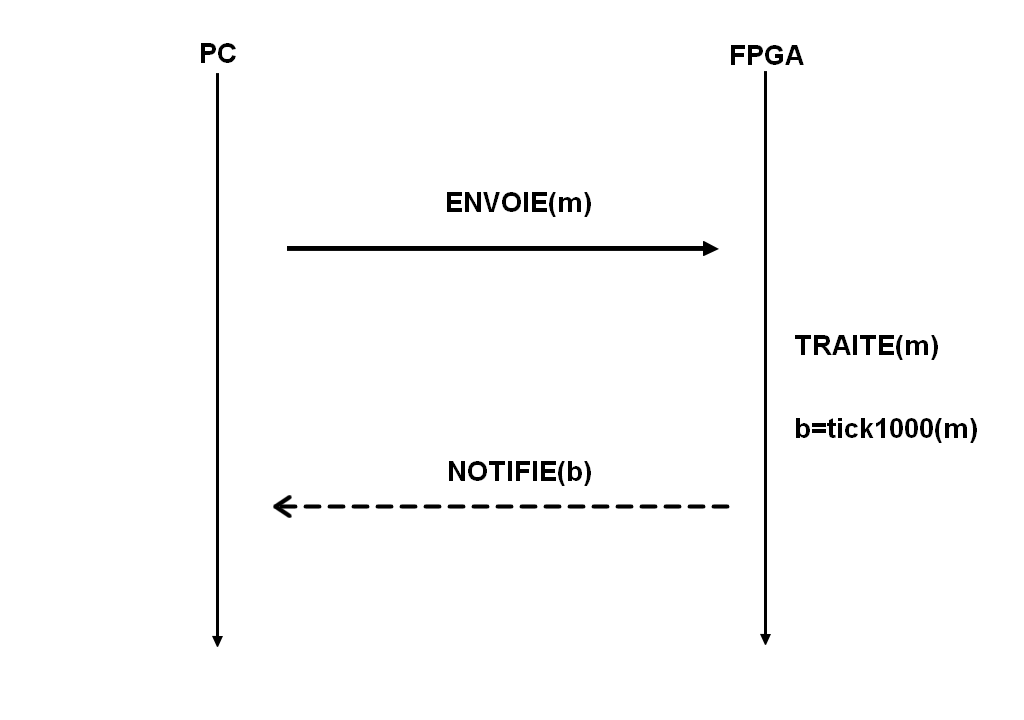
\includegraphics[width=7cm]{fonctionnement.png}
            \caption{MSC des actions utilisateur}
        \end{figure}
        
        \textbf{m} est un \textit{message}. Il s'agit d'une suite de \textbf{44 bits} avec le format:
        
        - \textbf{bits 43 à 24} Ce sont les bits du contrôle du BUS-IA (voir Bus-IA)
        
        - \textbf{bits 23 à 0} Ce sont les bits du message
        \newline
        \newline
        Un \textit{message} doit avoir le format:
        
        - \textbf{bits 23 à 21} Ce sont les bits coddant le \textit{type} du \textit{message}
        
        - \textbf{bits 20 à 0} Ce sont les données du message, le format varie selon le \textit{type}
        
        \subsection{Format des messages}
        
        Ci-dessous, voici les commandes supportées par le processeur,
        et le format des messages permettant d'executer ces commandes.
        \newline
        \newline
        \textbf{noop} Ne rien faire
        
        - \textbf{bits 23 à 21} : ``000'' (= (bit 23, bit 22, bit 21))

        - \textbf{bits 20 à 0} : \textit{non utilisées}
        \newline
        \newline
        \textbf{h-init(n)} Génère un tick sur H100 tous les n coups d'horloge maître
        
        - \textbf{bits 23 à 21} : ``001''

        - \textbf{bits 20 à 0} : \textit{non utilisées}
        \newline
        \newline
        \textbf{h-check-ON()} Demande au processeur d'envoyer au PC un message TICK1000 tous les 1000 tickets de H100.
        
        - \textbf{bits 23 à 21} : ``010''

        - \textbf{bits 20 à 0} : \textit{non utilisées}
        \newpage
        \textbf{h-check-OFF()} Demande au processeur d'arrêter d'envoyer au PC un message TICK1000
        
        - \textbf{bits 23 à 21} : ``011''

        - \textbf{bits 20 à 0} : \textit{non utilisées}
        \newline
        \newline
        \textbf{clr()} Indique au processeur d'afficher un serpentin vide sur le 7-segment (\textbf{n} à 32 et met à 0 toutes les \textit{valeurs} programmées
        
        - \textbf{bits 23 à 21} : ``100''

        - \textbf{bits 20 à 0} : \textit{non utilisées}
        \newline
        \newline
        \textbf{set-N(n)} Indique au processeur le nombre de \textbf{valeurs} à faire défiler en boucle sur le 7-segments. (\textbf{n} compris entre 1 et 32)
        
        - \textbf{bits 23 à 21} : ``101''

        - \textbf{bits 20 à 6} : \textit{non utilisées} 

        - \textbf{bits 5 à 0} : \textbf{n} coddé sur 6 bits ($2^6 = 64$)
        \newline
        \newline
        \textbf{set-val(i, v)} Indique au processeur la i-ème valeur du 7-segments est \textbf{v}
        
        - \textbf{bits 23 à 21} : ``110''

        - \textbf{bits 20 à 13} : \textit{non utilisées} 

        - \textbf{bits 12 à 6} : \textbf{v} les 7 bits correspond aux 7 segments de l'afficheur (0 => éteinds, 1 => allumé)

        - \textbf{bits 5 à 0} : \textbf{n} coddé sur 6 bits ($2^6 = 64$)

    \newpage
    \section{Description matérielle}
    
    \newpage
    \section{Présentation générale}
        \subsection{Schéma général}
        \subsection{Description des blocs}
        
    \newpage
    \section{Implémentation du bloc ????}
    
    
\end{document}
